\documentclass[tikz,border=10pt]{standalone}
\usepackage{tikz}
\usetikzlibrary{arrows.meta,patterns,decorations.pathmorphing}

\begin{document}
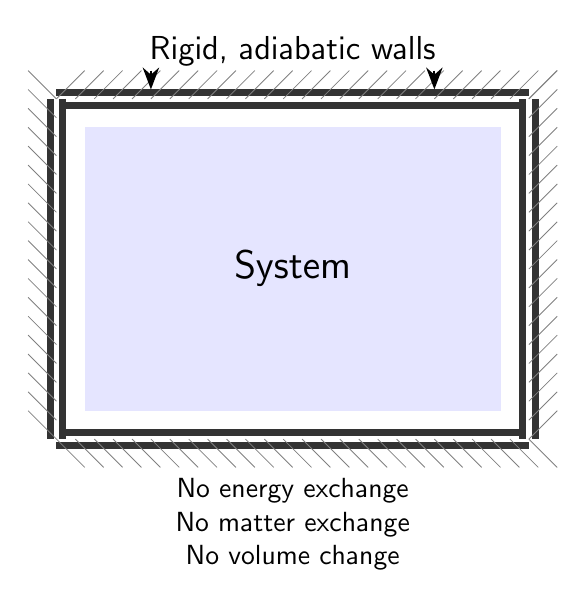
\begin{tikzpicture}[scale=1.2]

    % Define styles
    \tikzset{
        rigid wall/.style={line width=2.5pt, double distance=2pt, draw=black!80},
        system box/.style={fill=blue!10, draw=none},
        label/.style={font=\Large\sffamily}
    }

    % Define coordinates for the outer boundary (universe boundary - implicit)
    \coordinate (univ-nw) at (-3.5, 2.5);
    \coordinate (univ-ne) at (3.5, 2.5);
    \coordinate (univ-sw) at (-3.5, -2.5);
    \coordinate (univ-se) at (3.5, -2.5);

    % Define coordinates for the rigid wall boundary
    \coordinate (wall-nw) at (-2.5, 1.8);
    \coordinate (wall-ne) at (2.5, 1.8);
    \coordinate (wall-sw) at (-2.5, -1.8);
    \coordinate (wall-se) at (2.5, -1.8);

    % Define coordinates for the system interior
    \coordinate (sys-nw) at (-2.2, 1.5);
    \coordinate (sys-ne) at (2.2, 1.5);
    \coordinate (sys-sw) at (-2.2, -1.5);
    \coordinate (sys-se) at (2.2, -1.5);

    % Draw the system interior (light blue fill)
    \fill[system box] (sys-sw) rectangle (sys-ne);

    % Draw the rigid walls (thick double lines)
    % Top wall
    \draw[rigid wall] (wall-nw) -- (wall-ne);
    % Bottom wall
    \draw[rigid wall] (wall-sw) -- (wall-se);
    % Left wall
    \draw[rigid wall] (wall-nw) -- (wall-sw);
    % Right wall
    \draw[rigid wall] (wall-ne) -- (wall-se);

    % Add diagonal hatching pattern to indicate rigid/adiabatic walls
    \foreach \x in {-2.5,-2.3,...,2.5} {
        \draw[line width=0.3pt, gray] (\x, 1.8) -- (\x+0.3, 2.1);
        \draw[line width=0.3pt, gray] (\x, -1.8) -- (\x+0.3, -2.1);
    }
    \foreach \y in {-1.8,-1.6,...,1.8} {
        \draw[line width=0.3pt, gray] (-2.5, \y) -- (-2.8, \y+0.3);
        \draw[line width=0.3pt, gray] (2.5, \y) -- (2.8, \y+0.3);
    }

    % Label the system
    \node[label] at (0, 0) {System};

    % Label the rigid walls with arrows
    \node[font=\large\sffamily] at (0, 2.3) {Rigid, adiabatic walls};
    \draw[-{Stealth[scale=1.2]}, thick] (-1.5, 2.1) -- (-1.5, 1.9);
    \draw[-{Stealth[scale=1.2]}, thick] (1.5, 2.1) -- (1.5, 1.9);

    % Add annotations for constraints
    \node[font=\normalsize\sffamily, align=center] at (0, -2.7) {
        No energy exchange\\
        No matter exchange\\
        No volume change
    };

\end{tikzpicture}
\end{document}
